\begin{figure}[h!]
  \centering
  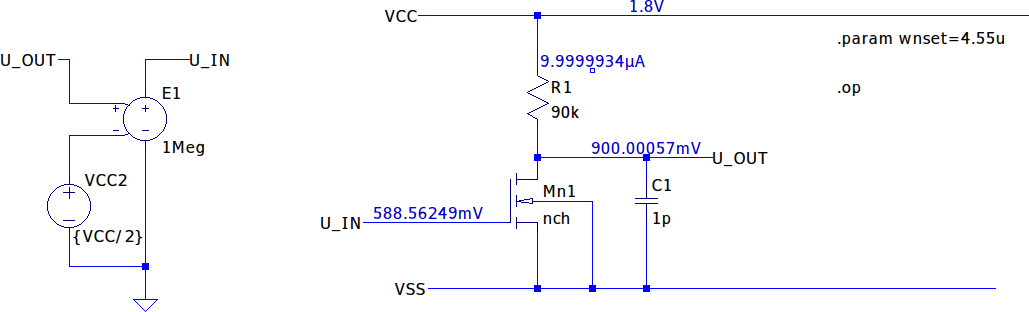
\includegraphics[scale=0.5]{4-1-1.png}
  \caption{Odporová zátěž -- zapojení pro OP analýzu.}
  \label{fig:spice0-png}
\end{figure}
\begin{figure}[h!]
    \centering
    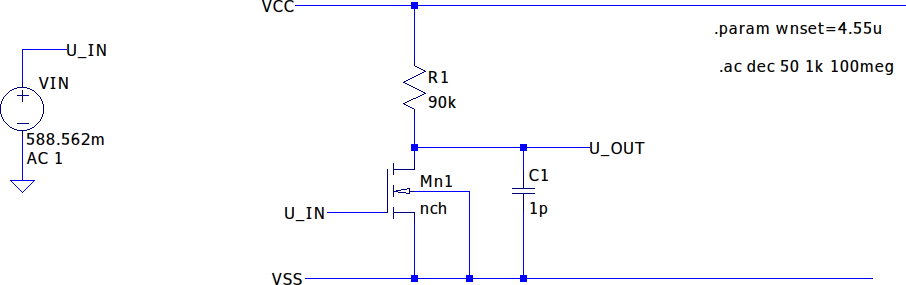
\includegraphics[scale=0.5]{4-1-2.png}
    \caption{Odporová zátěž -- zapojení pro AC analýzu.}
    \label{fig:spice0-png}
  \end{figure}
  \begin{figure}[h!]
    \centering
    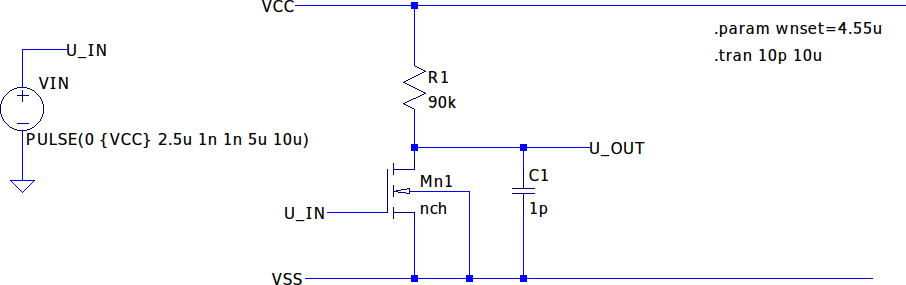
\includegraphics[scale=0.5]{4-1-3.png}
    \caption{Odporová zátěž -- zapojení pro TRAN analýzu.}
    \label{fig:spice0-png}
  \end{figure}


\subsubsection{Ruční návrh}
    Jako první krok je potřeba stanovit proud obvodem. Vyjdeme z požadovaných parametrů zapojení:
    \begin{align*}
        SR & =\frac{I_D}{C_{OUT}} \\
        I_{D-SR}  & =SR\cdot C_{OUT} \\
        I_{D-SR}  & =\num{10e6}\cdot \num{1e-12} \\
        I_{D-SR}  & =\qty{10}{\micro\ampere} 
    \end{align*}
    
    \begin{align*}
        GBW & =\frac{g_{m 1}}{2 \cdot \pi \cdot C_{O U T}}=\frac{\frac{2 \cdot I_D}{U_{O V}}}{2 \cdot \pi \cdot C_{O U T}} \\
        I_{D-GBW}  & =GBW\cdot \pi \cdot C_{OUT} \cdot U_{OV} \\
        I_{D-GBW}  & =\num{10e6}\cdot \pi \cdot \num{1e-12} \cdot \num{0.2} \\
        I_{D-GBW}  & =\qty{6.28}{\micro A}
    \end{align*}


    Zvolíme vyšší z vypočtených hodnot, tedy proud naším zapojením \(I_{D} = I_{D-SR} = \qty{10}{\micro\ampere} \). Pro rozměry tranzistoru je ještě potřeba zohlednit požadavek na zesílení, který nám stanoví maximální povolenou hodnotu \(\lambda_{max}  \):
    
    \begin{align*}
        A_{U 0} & =\frac{2}{U_{O V}} \cdot \frac{U_{C C}}{U_{C C} \cdot \lambda_{max} +2} \\
        A_{U 0} \cdot (U_{C C} \cdot \lambda_{max} +2) & =\frac{2}{U_{O V}} \cdot \frac{U_{C C}}{1} \\
        \lambda_{max} & =\frac{\frac{2\cdot U_{C C}}{U_{O V}} -2\cdot A_{U0}}{U_{CC}\cdot A_{U0}  } \\
        \lambda_{max} & =\frac{\frac{2\cdot \num{1.8}}{\num{0.2}} -2\cdot 10^{\frac{20}{20}}}{\num{1.8}\cdot 10^{\frac{20}{20}}} \\
        \lambda_{max} & =\qty{}{}
    \end{align*}
    


Nejprve vypočítám rozměry pro tranzistor \(M_{1} \):
\[
    \frac{W_{1} }{L}=\frac{2\cdot I_{D}}{KP_{N}\cdot (U_{GS} -U_{TH})^2 } 
\]
\[
    \frac{W_{1} }{L}=\frac{2\cdot \num{10e-6}}{\num{220e-6}\cdot (\num{0.2})^2 } 
\]

\[
    \frac{W_{1} }{L}\doteq \num[round-mode=places,round-precision=2]{2.27} 
\]
Délku \(L\) zvolíme opět \qty{2}{\micro\meter}, tedy \(W_{1}= \qty{4.55}{\micro\meter}\).

Pro velikost rezistoru \(R1\) je předpokládáno na výstupu napětí rovno polovině napájecího napětí, tedy platí:
\begin{align*}
    R_{1}  &= \frac{\frac{U_{CC}}{2}}{I_{D} } \\
    R_{1}  &= \frac{\frac{\num{1.8}}{2}}{\num{10e-6} } \\
    R_{1}  &= \qty{90}{k\ohm} \\
\end{align*}



\subsubsection{Očekávané hodnoty}
    Na základě zvolených parametrů součástek je potřeba přepočítat některé hodnoty. Proud \(I_{D} = \qty{10}{\micro A}\) byl zvolen pro \(SR=\qty{10}{V\per\micro\second}\), tímto se ale změní \(GBW\):
    \begin{align*}
        GBW & =\frac{\frac{2 \cdot I_D}{U_{O V}}}{2 \cdot \pi \cdot C_{O U T}} \\
        GBW & =\frac{\frac{2 \cdot \num{10e-6}}{\num{0.2}}}{2 \cdot \pi \cdot \num{1e-12}} \\
        GBW & =\qty{15.915}{MHz} \\
    \end{align*}

    Z rozměrů tranzistoru a tabulky z první úlohy odhadneme \(\lambda=\qty{0.0437895}{\per V}\), tedy očekáváme:
    \begin{align*}
        A_{U 0} & =\frac{2}{U_{O V}} \cdot \frac{U_{C C}}{U_{C C} \cdot \lambda_{max} +2} \\
        A_{U 0} & =\frac{2}{\num{0.2}} \cdot \frac{\num{1.8}}{\num{1.8} \cdot \num{0.0437895} +2} \\
        A_{U 0} & = \num{8.659} = \qty{18.749}{dB}
    \end{align*}




\subsubsection{Simulace}
    Z analýzy OP zjistíme optimální hodnotu \(U_{GS} = \qty{588,562}{mV}\) 
    % --- Operating Point ---

    % V(vcc):	 1.8	 voltage
    % V(u_out):	 0.900001	 voltage
    % V(u_in):	 0.588562	 voltage
    % V(n001):	 0.9	 voltage
    % Id(Mn1):	 9.99999e-06	 device_current
    % Ig(Mn1):	 0	 device_current
    % Ib(Mn1):	 -9.10001e-13	 device_current
    % Is(Mn1):	 -9.99999e-06	 device_current
    % I(C1):	 9.00001e-25	 device_current
    % I(R1):	 9.99999e-06	 device_current
    % I(E1):	 0	 device_current
    % I(Vcc):	 -9.99999e-06	 device_current
    % I(Vcc2):	 0	 device_current

\begin{figure}[h!]
    \centering
    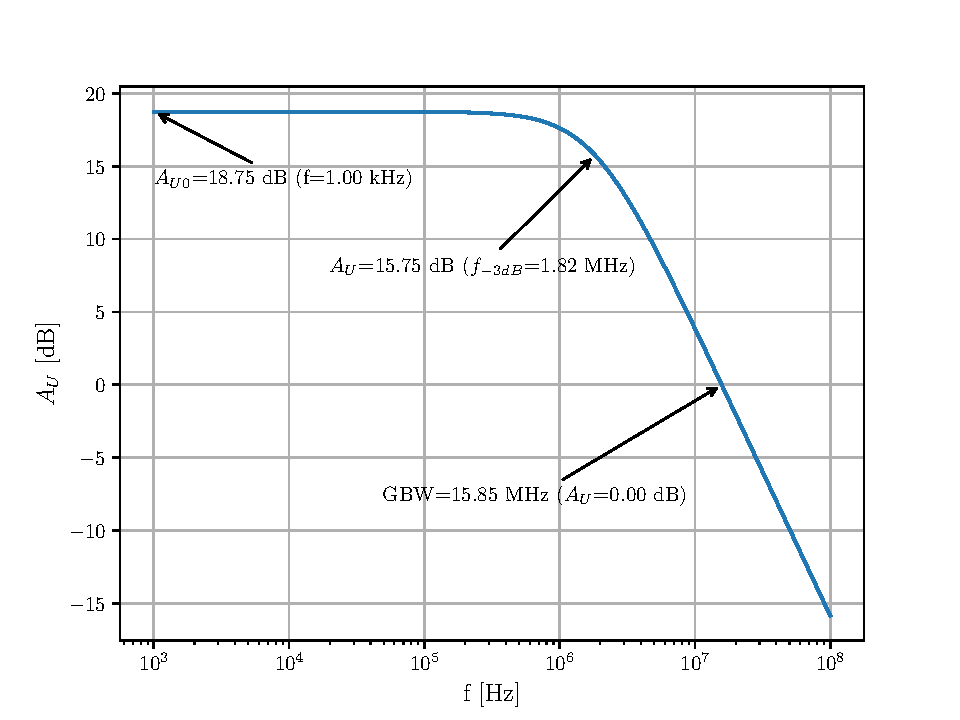
\includegraphics[width=0.8\textwidth]{4-1-2.pdf}
    \caption{AC analýza pro zesilovač s odporovou zátěží.}
    \label{fig:2-2-pdf}
\end{figure}

Kontrolní výpočet GBW ze simulovaných hodnot:
\begin{align*}
    GBW &= A_{0}\cdot f_{-3dB} \\
    GBW &= 10^{\frac{\num{18.75}}{20}}\cdot \num{1.82e6} \\
    GBW &= \qty{15.761}{MHz}\\
\end{align*}

\begin{figure}[h!]
    \centering
    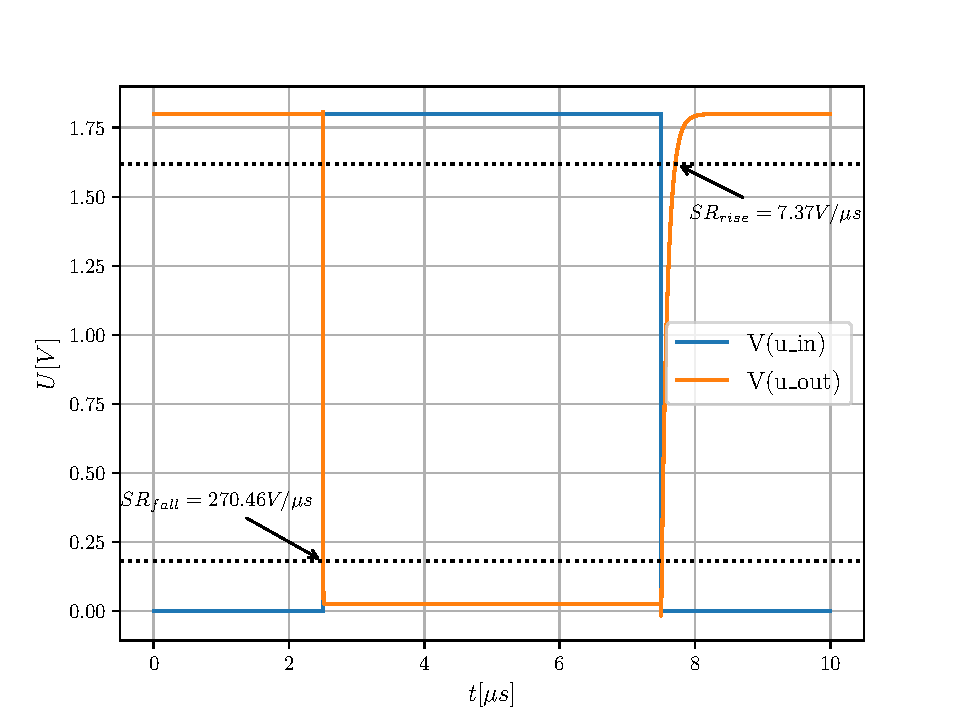
\includegraphics[width=0.8\textwidth]{4-1-3.pdf}
    \caption{TRAN analýza pro zesilovač s odporovou zátěží.}
    \label{fig:2-2-pdf}
\end{figure}

